\documentclass[
  aps,
  pra,
  reprint,
  superscriptaddress,
  longbibliography,
  nofootinbib
]{revtex4-2}

% ============================================================
% Encoding and typography
% ============================================================
\usepackage[T1]{fontenc}
\usepackage[utf8]{inputenc}
\usepackage{microtype}

% ============================================================
% Mathematics
% ============================================================
\usepackage{amsmath,amssymb,amsfonts}
\usepackage{bm}

% ============================================================
% Figures, tables, and floats
% ============================================================
\usepackage{graphicx}
\graphicspath{{figures/}}
\usepackage{booktabs}
\usepackage{array}
\usepackage{multirow}
\usepackage{placeins}

% ============================================================
% Table rule styling
% ============================================================
% Every table defines its own font size, column padding, row spacing, and
% resize target locally. Keeping those controls beside each table makes the
% layout easy to tune without hidden global sizing behavior.
\setlength{\heavyrulewidth}{0.10pt}
\setlength{\lightrulewidth}{0.10pt}
\setlength{\cmidrulewidth}{0.10pt}
\setlength{\arrayrulewidth}{0.10pt}
\setlength{\aboverulesep}{1pt}
\setlength{\belowrulesep}{1pt}

% ============================================================
% Algorithms and code
% ============================================================
\usepackage{algpseudocode}

% ============================================================
% Units, colors, links, and references
% ============================================================
\usepackage[table,dvipsnames]{xcolor}

% Table-only colors. Keep fills deliberately light for print readability.
% The proposed method is highlighted cell-by-cell (not with \rowcolor), so
% the tint cannot leak into following rows or obscure group labels.
\definecolor{proposedrow}{RGB}{234,242,250}
\definecolor{gaincol}{RGB}{137,190,132}
\definecolor{losscol}{RGB}{224,132,132}
\definecolor{neutralcol}{RGB}{242,242,242}
\newcommand{\proposedcell}[1]{\cellcolor{proposedrow}#1}
\newcommand{\proposedbest}[1]{\cellcolor{proposedrow}\textbf{#1}}
\usepackage{xurl}

% REVTeX 4.2 redefines \label. Modern nameref (loaded by hyperref)
% detects and repairs that definition, but emits a known compatibility warning.
% Silence only that specific warning; all other warnings remain visible.
\usepackage{silence}
\WarningFilter{nameref}{The definition of \label has changed}

\usepackage{hyperref}
\usepackage[nameinlink,capitalise,noabbrev]{cleveref}
\setcitestyle{numbers,square,comma}

\hypersetup{
  colorlinks=true,
  linkcolor=MidnightBlue,
  citecolor=MidnightBlue,
  urlcolor=MidnightBlue,
  pdfauthor={Research Hub team},
  pdftitle={Listening to Silence: Attention Sinks, Registers, and the Hidden Work of Padding in Speech Transformers}
}

% ============================================================
% Convenience macros
% ============================================================
\newcommand{\method}{\textsc{SilenceCache}}
\newcommand{\R}{\mathbb{R}}
\newcommand{\E}{\mathbb{E}}
\newcommand{\norm}[1]{\left\lVert #1 \right\rVert}
\newcommand{\vect}[1]{\bm{#1}}
\newcommand{\secref}[1]{\hyperref[#1]{\S\ref*{#1}}}
\newcommand{\figref}[1]{Fig.~\ref{#1}}
\newcommand{\tabref}[1]{Table~\ref{#1}}
\newcommand{\eqnref}[1]{Eq.~\eqref{#1}}
\newcommand{\appref}[1]{\hyperref[#1]{\S\ref*{#1}}}
\newcommand{\guide}[1]{\par\noindent\textit{Writing guide.}~#1\par}

% Theorem-style environments in REVTeX
\newtheorem{theorem}{Theorem}
\newtheorem{lemma}{Lemma}
\newtheorem{proposition}{Proposition}
\newtheorem{definition}{Definition}
\newenvironment{proof}{\par\noindent\textit{Proof.}\ }{\hfill$\square$\par}

\begin{document}

% ============================================================
% Title block -- full width above the two-column body
% ============================================================
\title{Listening to Silence: Attention Sinks, Registers, and the Hidden Work of Padding in Speech Transformers}

% Author block: placeholders -- fill in names, e-mails and affiliations before sharing.
\author{Author One}
\email{author.one@example.edu}
\affiliation{Department, Institution, City, Country}

\author{Author Two}
\affiliation{Department, Institution, City, Country}

\author{Author Three}
\affiliation{Department, Institution, City, Country}


\begin{abstract}
Whisper, the most widely deployed speech recognizer and the audio encoder inside many audio language models, always pads its input to 30\,s, and it fails when the padding is removed: in our pilot, word error rate (WER) on short LibriSpeech utterances rises from 5.3\% to 373\% for Whisper-base and from 2.0\% to 428\% for Whisper-large-v3-turbo, mostly through runaway repetition. Existing fixes retrain the model or a learned input segment, and the role of the silent frames is not understood. We study what speech transformers do with silence through the lens of attention sinks, massive activations and register tokens---phenomena with competing 2026 theories that have been examined in language and vision models but not in speech encoders. In three Whisper sizes the encoder forms textbook high-norm, massive-activation tokens on the padding, yet these tokens are dispensable for recognition: masking or removing them leaves WER unchanged. What Whisper needs is silence used in two ways: decoder cross-attention to silent encoder states as end-of-speech evidence, and encoder self-attention to a few position-anchored sink frames at the edges of the 30\,s window. In large-v3-turbo, 16 cached high-attention silence frames give 2.6\% WER versus 17.5\% for 16 random ones. Building on this, \method{} precomputes silence keys, values and outputs once and encodes only the speech; it matches or improves full-padding WER (5.1/2.6/1.7\% vs.\ 5.3/2.6/2.0\%) at 0.16$\times$ the encoder FLOPs, without any training. These numbers come from a 100-utterance pilot; the full evaluation is specified in Sec.~\ref{sec:evaluation}.
\end{abstract}

\maketitle

% ============================================================
% Paper body -- each major section is maintained separately
% ============================================================
% ============================================================
% 01. INTRODUCTION
% ============================================================
\section{Introduction}
\label{sec:intro}

Whisper~\cite{radford2023whisper} processes every input as a 30\,s window. A two-second voice command is zero-padded with 28\,s of digital silence before the encoder runs, so roughly 90\% of the encoder computation is spent on frames that carry no signal. Removing the padding is the obvious fix, and it fails badly. On 100 short LibriSpeech~\cite{panayotov2015librispeech} utterances (2--8\,s), feeding only the speech frames raises greedy-decoding WER from 5.3\% to 373\% for Whisper-base, from 2.6\% to 214\% for Whisper-small and from 2.0\% to 428\% for Whisper-large-v3-turbo; most outputs loop on the last phrase (Table~\ref{tab:results}). Because Whisper's encoder is also the audio front-end of many audio language models, the cost of the padding, and of not understanding it, propagates widely.

Current remedies treat the padding as an engineering obstacle. WhisperFlow trains a 0.5\,s ``hush word'' appended to the audio~\cite{wang2024whisperflow}; WhisperKit self-distils the encoder with block-diagonal masks so that a silent block can be cached~\cite{orhon2025whisperkit}; other systems detect and truncate hallucinated continuations online~\cite{lee2026npusper} or drop encoder tokens~\cite{cho2026stridek}. Each of these either retrains something or works around the failure without explaining it. The basic question remains open: \emph{what does a speech transformer compute with 28\,s of silence?}

A natural hypothesis comes from the literature on attention sinks, massive activations and register tokens. Vision transformers recruit uninformative background patches as high-norm ``registers'' that store global information~\cite{darcet2024registers,jiang2025testtime}; language models dump attention on the first token, whose massive activations act as implicit biases~\cite{sun2024massive,xiao2024streaming}. These phenomena are among the most actively studied transformer mechanisms in 2026, with competing accounts of why they arise and whether they matter: pre-normalisation makes sinks and massive activations co-occur but each can exist without the other~\cite{sun2026anatomy}; sinks stem from the unaggregated first token under causal masking~\cite{li2026structural}; softmax attention needs a sink to implement a default ``no-op'' state~\cite{ranmilo2026necessary}; spikes land on the least-shared token~\cite{ngnawe2026spike}; or high-norm artifacts are a symptom of lazy aggregation rather than the cause~\cite{shi2026lastvit}. None of this work examines speech encoders, where ``nothing'' is not a rare background patch but a large, exactly controllable part of every input.

We examine Whisper through this lens and find a sharper picture than the register hypothesis predicts. Whisper's encoder does form textbook registers on the padding: a few frames reach 29--59$\times$ the median token norm, and in Whisper-base and -small they carry massive activations above Sun et~al.'s threshold~\cite{sun2024massive} (Whisper-base: a single activation of 501, 1{,}122$\times$ the median magnitude). But they are \emph{dispensable}: masking encoder attention to them, or removing them from the decoder's view, leaves WER unchanged in all three models. What Whisper actually needs is \emph{silence}, used in two ways. First, the decoder needs silent encoder states as end-of-speech evidence; without them it loops. Second, the encoder's speech frames attend to a handful of \emph{attention-sink} frames that sit at fixed positions near the start and end of the 30\,s window. These two roles can be supplied without encoding any padding: a content-free silence input is encoded once, its keys, values and outputs are cached, and each utterance is encoded alone while attending to the cache. We call this \method{}. In the pilot it matches or improves full-padding WER at 0.16$\times$ the encoder FLOPs, and its reliance on the sink frames grows with model size: for large-v3-turbo, caching the 16 most-attended silence frames recovers 2.6\% WER, while 16 random silence frames give 17.5\% (Fig.~\ref{fig:topk}).

\paragraph{Contributions.}
(i)~A protocol and census of registers, massive activations and attention sinks in speech and audio encoders, with natural experiments over normalisation type, special tokens and padding regime (visible in Whisper, masked in Whisper-derived audio-LLM encoders, absent in windowed encoders). (ii)~Controlled acoustic interventions that pit the 2026 accounts of sink formation against each other by varying the energy, redundancy, position and duration of non-speech input. (iii)~Causal evidence, in production speech models, that functional attention sinks and high-norm registers dissociate, together with an anatomy of how the decoder uses silence to stop. (iv)~\method{}, a training-free method for padding-free Whisper that follows from this mechanism, benchmarked against trained alternatives. Items (i)--(iii) are supported by pilots reported here; the full-scale evaluation is specified in Sec.~\ref{sec:evaluation}, and the evidence log behind every claim is maintained in the project repository.

% ============================================================
% 02A. BACKGROUND
% ============================================================
\section{Background}
\label{sec:background}

\subsection{Problem Setting}

\paragraph{Whisper's input window.} An utterance $x$ of duration $\tau\le 30$\,s is converted to an 80- or 128-channel log-mel spectrogram with a 10\,ms hop and zero-padded to 3000 frames; a two-layer convolutional stem (second layer stride 2) yields $N=1500$ encoder positions, to which fixed sinusoidal position embeddings $\mathbf{p}_1,\dots,\mathbf{p}_N$ are added~\cite{radford2023whisper}. The encoder is a stack of $L$ pre-normalisation (pre-LN) transformer blocks followed by a final LayerNorm; every Whisper size uses 64-dimensional attention heads (tiny: 4 layers, width 384; large: 32 layers, width 1280). Let $T=\lceil 50\tau\rceil$ be the number of positions covered by speech. With padding, positions $T{+}1,\dots,N$ hold the encoding of digital silence; the decoder cross-attends to all $N$ encoder outputs $\mathbf{H}=[\mathbf{h}_1,\dots,\mathbf{h}_N]$.

\paragraph{Goal.} We ask which computations the padded positions perform, and whether those computations can be supplied when the encoder processes only the $T$ speech positions. The task performance measure is the word error rate of the decoded transcript,
\begin{equation}
    \mathrm{WER}
    = \frac{S+D+I}{N_{\mathrm{ref}}},
    \label{eq:objective}
\end{equation}
with substitutions $S$, deletions $D$ and insertions $I$ against $N_{\mathrm{ref}}$ reference words after Whisper's text normaliser. Because insertions are unbounded, WER exceeds 100\% when the decoder loops; we therefore also report a hallucination rate (Sec.~\ref{sec:metrics}). All interventions are applied at inference time to frozen public checkpoints; no parameter is trained.

\subsection{Notation and Preliminaries}

For a layer $\ell$ with hidden states $\mathbf{X}^{(\ell)}\in\R^{N\times d}$, a head with queries $\mathbf{q}_i$, keys $\mathbf{k}_j$ and values $\mathbf{v}_j$ computes
\begin{equation}
    \mathbf{o}_i = \sum_{j} a_{ij}\mathbf{v}_j,\qquad
    a_{ij}=\frac{\exp(\mathbf{q}_i^\top\mathbf{k}_j)}{\sum_{m}\exp(\mathbf{q}_i^\top\mathbf{k}_m)}.
    \label{eq:loss}
\end{equation}
We use three observables that recent work shows can dissociate~\cite{sun2026anatomy,ngnawe2026spike}.

\begin{definition}[Register frame, massive activation, attention sink]
A \emph{register (high-norm) frame} at layer $\ell$ is a position whose hidden-state norm exceeds ten times the median token norm, $\norm{\mathbf{x}^{(\ell)}_j}_2>10\,\mathrm{med}_m\norm{\mathbf{x}^{(\ell)}_m}_2$. A \emph{massive activation} is a single entry with $|x^{(\ell)}_{jc}|>100$ that is at least about $1000\times$ the median entry magnitude of the layer~\cite{sun2024massive}; we report the ratio $\Psi^{(\ell)}=\max_{j,c}|x_{jc}|/\mathrm{med}_{j,c}|x_{jc}|$. An \emph{attention-sink frame} is a position whose received attention, averaged over heads and queries, $\bar a_j=\frac{1}{HN}\sum_{h,i}a^{h}_{ij}$, is among the largest in the layer; following Gu et~al.~\cite{gu2025sinkemerges}, a sink holds at least 30\% of the attention mass in some layer.
\end{definition}

The following elementary fact explains why a sink can implement a ``no-op'' and why sink keys and values can be cached.

\begin{proposition}
\label{prop:placeholder}
Fix a head and a query $\mathbf{q}_i$. Suppose one key $\mathbf{k}_s$ satisfies $\mathbf{q}_i^\top\mathbf{k}_s-\max_{j\neq s}\mathbf{q}_i^\top\mathbf{k}_j\ge\Delta$ and all values are bounded, $\norm{\mathbf{v}_j}_2\le V$. Then
\begin{equation}
    \norm{\mathbf{o}_i-\mathbf{v}_s}_2 \le 2V\,(n-1)\,e^{-\Delta},
    \label{eq:placeholder-bound}
\end{equation}
where $n$ is the number of keys. Hence, as the logit gap grows, the head output tends to the constant $\mathbf{v}_s$, independent of the content of the other tokens.
\end{proposition}

\begin{proof}
$1-a_{is}=\sum_{j\ne s}a_{ij}\le(n-1)e^{-\Delta}$ and $\mathbf{o}_i-\mathbf{v}_s=\sum_{j\ne s}a_{ij}(\mathbf{v}_j-\mathbf{v}_s)$, whose norm is at most $2V(1-a_{is})$.
\end{proof}

Proposition~\ref{prop:placeholder} is the reason a sink acts as an attention bias~\cite{sun2024massive,jiang2025testtime}: what matters for the other tokens is the sink's key and value, not where they were computed. If the keys and values of the silent positions do not depend on the utterance, they can be computed once and reused. Sec.~\ref{sec:method} tests how far this holds for Whisper.

% ============================================================
% 02B. RELATED WORK
% ============================================================
\section{Related Work}
\label{sec:related}

\subsection{Closest Methodological Line}

\paragraph{Registers, sinks and massive activations.} High-norm artifact tokens in vision transformers were linked to redundant background patches and global information and removed by training with extra register tokens~\cite{darcet2024registers}. Test-time registers move them into an added token by editing a sparse set of ``register neurons'' without training~\cite{jiang2025testtime}, and RegCache prefixes cached register keys and values to suppress activation outliers for quantization~\cite{kim2026regcache}. In language models, attention sinks on the first token enable streaming~\cite{xiao2024streaming}, and massive activations act as fixed biases~\cite{sun2024massive}. The 2026 literature disputes the mechanism: pre-normalisation couples sinks and massive activations but either can be removed without loss~\cite{sun2026anatomy}; sinks arise from the first token's unaggregated variance under causal masking~\cite{li2026structural}; massive activations emerge in a single layer~\cite{shi2026melayer} and cause compression valleys~\cite{queipo2026valleys}; sinks are provably needed for default states~\cite{ranmilo2026necessary}; outlier-driven rescaling is essential for training~\cite{qiu2026residualsinks}; and gating removes sinks~\cite{qiu2025gated}. In vision, artifacts are attributed to lazy aggregation~\cite{shi2026lastvit}, and high-norm tokens were not found in bidirectional text encoders~\cite{wang2025singular}. All of this work concerns text, images or diffusion models; none studies speech encoders, silence or fixed-length padding.

\paragraph{Sinks at the encoder--LLM interface.} High-norm ViT tokens propagate into vision-language models and carry global semantics~\cite{luo2026sink}; visual massive activations in LVLMs are brittle and follow a least-shared location rule~\cite{ngnawe2026spike}. For audio, sinks have been characterised only inside the language model of audio-visual LLMs~\cite{anand2026avsrsinks,jung2026hubs,yoo2026omni}, and audio-token attention has been predicted from encoder outputs for pruning~\cite{park2026triage}. The audio encoder itself, and in particular its silent frames, is not analysed in any of these works.

\subsection{Complementary Research Direction}

\paragraph{Efficient and padding-free Whisper.} Short inputs make Whisper hallucinate, so streaming systems pad and overlap buffers. WhisperFlow appends a trained 0.5\,s audio ``hush word''~\cite{wang2024whisperflow}; WhisperKit self-distils block-diagonal attention so that a silent block's encoder output can be cached~\cite{orhon2025whisperkit}; NPUsper stops decoding when cross-attention moves backwards~\cite{lee2026npusper}; stride-$k$ subsampling drops encoder tokens without training~\cite{cho2026stridek}; Moonshine removes padding by retraining with rotary positions~\cite{jeffries2024moonshine}. Separately, a line of work mitigates Whisper's hallucinations on non-speech audio by masking heads~\cite{wang2025calmwhisper} or steering encoder representations~\cite{aparin2026whispersae}. These methods differ from ours in information access and cost: they require training data and optimisation, or address a different failure (non-speech input, decoding control), and none offers a mechanistic account of why padding is needed.

\subsection{Positioning of This Work}

The closest methods are test-time registers~\cite{jiang2025testtime} and RegCache~\cite{kim2026regcache}, which add or cache register tokens in vision encoders, and WhisperKit's silence caching~\cite{orhon2025whisperkit}, which reuses a silent block after retraining with block masks. We differ in three ways. First, we study speech encoders and their decoders, where the ``uninformative'' input is silence that can be manipulated exactly. Second, we separate functional attention sinks from high-norm registers in production models and find that only the former matter for recognition. Third, \method{} caches silence without retraining and without block masks: speech queries attend to cached silence keys and values, and the decoder sees a cached silence tail.

% ============================================================
% 03. METHOD
% ============================================================
\section{Method}
\label{sec:method}

\subsection{Overview}

Our study has two parts. The \emph{measurement and intervention protocol} records, for any frozen speech encoder, per-layer norms, activation magnitudes and received attention, labels each position as speech, in-utterance silence, padding or a fixed absolute position, and applies causal edits: masking attention to selected positions, removing positions from the decoder's view, and replacing computed keys, values and outputs with cached ones. The \emph{method}, \method{}, uses one of these edits as an inference procedure: it encodes a 30\,s silence input once, caches its per-layer keys and values and its final outputs, and then encodes each utterance without padding while letting speech queries attend to the cached silence and letting the decoder read a cached silence tail. The protocol is new in that it targets silence; \method{} is new in that it removes padding without training. Attention, normalisation and decoding are inherited unchanged from Whisper~\cite{radford2023whisper}.

\paragraph{Cached keys and values.} Let $\mathbf{K}^{(\ell)}_{\varnothing},\mathbf{V}^{(\ell)}_{\varnothing}\in\R^{N\times d}$ be the keys and values of layer $\ell$ and $\mathbf{S}=[\mathbf{s}_1,\dots,\mathbf{s}_N]$ the encoder outputs when the input is pure digital silence. For an utterance covering $T$ positions and a set $\mathcal{C}\subseteq\{T{+}1,\dots,N\}$ of cached positions, each speech query $\mathbf{q}_i$ ($i\le T$) attends over
\begin{align}
    \mathbf{K}_i^{(\ell)} &= \big[\mathbf{K}^{(\ell)}_{1:T};\ \mathbf{K}^{(\ell)}_{\varnothing,\mathcal{C}}\big], \\
    \mathbf{V}_i^{(\ell)} &= \big[\mathbf{V}^{(\ell)}_{1:T};\ \mathbf{V}^{(\ell)}_{\varnothing,\mathcal{C}}\big],
    \label{eq:update}
\end{align}
and the decoder cross-attends to $[\mathbf{H}_{1:T};\mathbf{S}_{\mathcal{D}}]$ for a set $\mathcal{D}$ of tail positions. With $\mathcal{C}=\mathcal{D}=\{T{+}1,\dots,N\}$ the only approximation relative to padded encoding is that the cached silence states were computed without the utterance in context (padding positions do not attend to speech). Restricting $\mathcal{C}$ to the $k$ silence positions with the largest received attention $\bar a_j$ in the silence-only run gives $\method{}$-top-$k$; drawing $\mathcal{C}$ uniformly at random gives the matched control.

\subsection{Framework Overview}

\begin{figure*}[t]
    \centering
    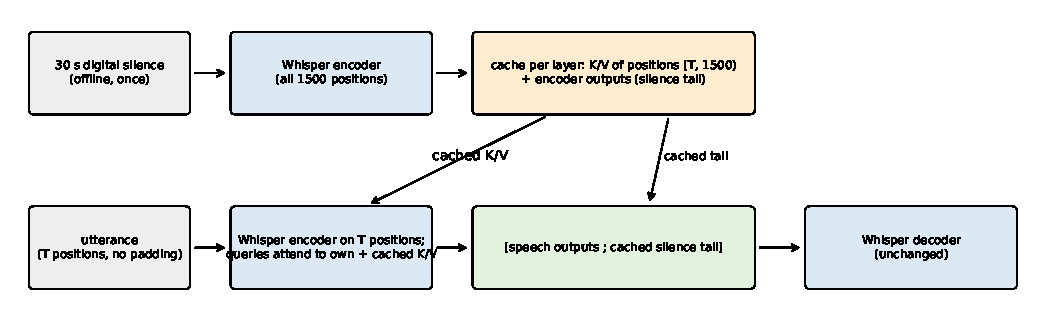
\includegraphics[width=\textwidth]{silencecache_overview.pdf}
    \caption{\method{} removes Whisper's padding without training. Offline (top), a 30\,s silence input is encoded once and its per-layer keys/values for positions $[T,1500)$ and its encoder outputs (the ``tail'') are cached. Online (bottom), only the $T$ speech positions are encoded; speech queries attend to their own keys plus the cached silence keys (all, or the top-$k$ attention sinks), and the unchanged decoder cross-attends to the speech states followed by the cached tail. Nothing is trained; the cost scales with $T$ rather than 1500 positions.}
    \label{fig:overview}
\end{figure*}

Figure~\ref{fig:overview} shows the inference path. The diagnostic variants used in Sec.~\ref{sec:evaluation} switch individual arrows off: \emph{tail only} ($\mathcal{C}=\emptyset$), \emph{KV only} ($\mathcal{D}=\emptyset$), top-$k$ versus random-$k$ caches, and a decoder that sees only the top-$k$ tail positions. Together they separate the encoder-side and decoder-side roles of silence.

\subsection{Core Components}

\begin{figure}[t]
    \centering
    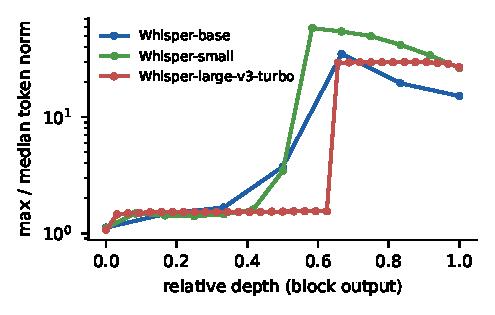
\includegraphics[width=\columnwidth]{norm_ratio_silence.pdf}
    \caption{Whisper's encoder forms high-norm register frames on silence. Max/median token norm per block output for a 30\,s silence input. The ratio jumps abruptly at one block (base: block 4 of 6; small: 7 of 12; large-v3-turbo: 20 of 32) and stays high, the single-layer emergence pattern reported for language models~\cite{shi2026melayer}.}
    \label{fig:single}
\end{figure}

\paragraph{Faithful forward pass.} We re-implement the Whisper encoder forward pass explicitly (convolutional stem, sinusoidal positions sliced to the input length, pre-LN blocks, final LayerNorm), so that inputs of any length and extra cached keys/values can be used. On a padded LibriSpeech utterance its output differs from the Hugging Face implementation by at most $6.9\times10^{-4}$ (output scale 23.6), and greedy decoding produces identical transcripts. Hidden states are recorded \emph{before} the final LayerNorm, because library conventions for returned hidden states differ across models and versions.

\paragraph{Observables.} Per layer we record the norm ratio, $\Psi^{(\ell)}$ and the absolute maximum activation, received attention per position, and, in the planned census, matrix entropy and anisotropy of $\mathbf{X}^{(\ell)}$~\cite{queipo2026valleys}. Positions are labelled with an energy voice-activity threshold ($-40$\,dBFS), with the padding boundary, and with absolute index.

\paragraph{Interventions.} (a) \emph{Encoder masking}: set the logits of selected key positions to $-\infty$ from a chosen block onwards. (b) \emph{Decoder removal}: delete selected positions from the encoder output before cross-attention. (c) \emph{Caching}: replace computed silence with cached keys, values and outputs as in Eq.~\eqref{eq:update}. Selections are either by norm (top-$k$ register frames at the emergence block) or by attention (top-$k$ sink frames in the silence-only run), with random-$k$ controls.

\subsection{Algorithm}

\begin{center}
\begin{minipage}{0.96\columnwidth}
\hrule\vspace{0.4em}
\textbf{Algorithm 1: \method{} inference}\vspace{0.25em}
\begin{algorithmic}[1]
\Require Whisper encoder/decoder; utterance $x$; cache size $k$ (or ``all'')
\State \textbf{Offline, once:} encode 30\,s of silence; store $\mathbf{K}^{(\ell)}_{\varnothing},\mathbf{V}^{(\ell)}_{\varnothing}$ for all layers, outputs $\mathbf{S}$, and received attention $\bar a_j$
\State Compute log-mel of $x$ without padding; $T\gets$ number of encoder positions
\State $\mathcal{C}\gets$ top-$k$ of $\{\bar a_j\}_{j>T}$ (or all $j>T$)
\For{$\ell=1,\ldots,L$}
    \State compute $\mathbf{Q},\mathbf{K},\mathbf{V}$ for the $T$ speech positions
    \State attend with keys/values $[\mathbf{K};\mathbf{K}^{(\ell)}_{\varnothing,\mathcal{C}}]$, $[\mathbf{V};\mathbf{V}^{(\ell)}_{\varnothing,\mathcal{C}}]$; MLP on $T$ positions
\EndFor
\State $\mathbf{H}\gets$ final LayerNorm output for the $T$ positions
\State \Return decode$\big([\mathbf{H};\mathbf{S}_{T+1:N}]\big)$
\end{algorithmic}
\vspace{0.3em}\hrule
\end{minipage}
\end{center}

\subsection{Complexity or Theoretical Analysis}

Counting multiply--accumulates as two FLOPs, one encoder layer with width $d$, MLP width $f=4d$, $T_q$ query positions and $T_k$ key positions costs
\begin{equation}
    C(T_q,T_k)=2T_q\,(4d^2+2df)+4\,T_q T_k d .
    \label{eq:cost}
\end{equation}
Padded inference costs $C(N,N)$ per layer. \method{} with a full cache costs $C(T,N)$ and with a top-$k$ cache $C(T,T{+}k)$. For Whisper-base ($d=512$) and a 4.7\,s utterance ($T\approx234$), $C(T,N)/C(N,N)\approx0.16$ and $C(T,T{+}16)/C(N,N)\approx0.11$, essentially the cost of no padding. Memory for the cache is $2Lkd$ values ($k=16$, large-v3: 1.3\,M values). Wall-clock speed-ups depend on kernels and batch size and are measured separately (Sec.~\ref{sec:setup}); the derivation of Eq.~\eqref{eq:cost} is in \appref{app:derivations}.

% ============================================================
% 04. EVALUATION
% ============================================================
\section{Evaluation}
\label{sec:evaluation}

We organise the evaluation around four research questions: \textbf{RQ1} where registers, massive activations and sinks form in speech encoders; \textbf{RQ2} which account of sink formation predicts their location; \textbf{RQ3} which of these structures Whisper needs, in the encoder and in the decoder; \textbf{RQ4} whether \method{} removes padding without loss. This draft reports the \emph{pilot} that motivated the study (three Whisper sizes, 100 utterances each) and specifies the full evaluation. Pilot numbers are marked as such and should be read as indicative.

\subsection{Experimental Setup}
\label{sec:setup}

The pilot uses the 100 LibriSpeech test-clean utterances with duration 2--8\,s selected by a fixed random seed (mean 4.7\,s), greedy decoding with the prompt \texttt{<|startoftranscript|><|en|><|transcribe|><|notimestamps|>}, a 160-token limit, and frozen public checkpoints. The full evaluation (planned) extends this to six Whisper sizes plus distil-large-v3, LibriSpeech test-clean/other in full, TED-LIUM~3, FLEURS in seven languages including Bengali, a short-command set, and noisy and long-form conditions; it adds wall-clock timing on T4 and RTX-3050 GPUs at batch sizes 1 and 16. The census for RQ1 covers about 18 checkpoints: Whisper, Moonshine (trained without padding~\cite{jeffries2024moonshine}), post-LN and pre-LN self-supervised encoders, AST with its CLS and distillation tokens~\cite{gong2021ast}, and the audio towers of audio language models that mask padding or use windows. Implementation details are listed in \appref{app:implementation}.

\begin{table}[!htbp]
\centering
\small
\setlength{\tabcolsep}{8pt}
\caption{Pilot configuration. Every value is fixed a priori; nothing is tuned on the test utterances.}
\label{tab:setup}
\begin{tabular}{l l}
\toprule
\textbf{Parameter} & \textbf{Setting} \\
\midrule
Dataset & LibriSpeech test-clean, 100 utts, 2--8\,s \\
Models & Whisper base, small, large-v3-turbo \\
Training & none (frozen checkpoints) \\
Decoding & greedy, English, no timestamps \\
Cache source & one 30\,s digital-silence input \\
Random seeds & 0 (utterances, random-$k$) \\
Hardware & RTX 3050 Laptop 4\,GB (fp32; turbo fp16) \\
\bottomrule
\end{tabular}
\end{table}

\subsection{Evaluation Metrics}
\label{sec:metrics}

WER follows Eq.~\eqref{eq:objective} after Whisper's English normaliser. Because looping transcripts inflate WER without bound, we also report the hallucination rate
\begin{equation}
    \mathrm{Hal}
    = \frac{1}{n}\sum_{i=1}^{n}
      \mathbf{1}\!\left[\,|\widehat{y}_i|>|y_i|+3\ \ \lor\ \ \mathrm{rep}(\widehat{y}_i)\right],
    \label{eq:accuracy}
\end{equation}
where $|\cdot|$ counts words and $\mathrm{rep}$ detects a three-word phrase repeated at least twice. Cost is reported as encoder FLOPs relative to padded inference (Eq.~\eqref{eq:cost}); the full evaluation adds measured latency, real-time factor and peak memory, and 95\% bootstrap confidence intervals with paired tests against padded inference.

\subsection{Main Results}
\label{sec:results}

Table~\ref{tab:results} compares padded inference, removal of padding, real partial padding and the \method{} variants on the same utterances. Three results stand out. First, removing padding is catastrophic for all sizes (WER 214--428\%), and real 5\,s padding is not a safe substitute: it is adequate for base and small but gives 35.1\% for large-v3-turbo. Second, the two roles of silence are separable and complementary. The cached tail alone fixes most loops for base and small but not for turbo (22.7\%), while cached keys and values alone do not prevent loops; together they match or improve padded WER in every model (5.12/2.64/1.71\% vs.\ 5.28/2.56/2.02\%) at 0.157$\times$ the encoder FLOPs. Third, removing high-norm register frames from the decoder's view, or masking encoder attention to them from the emergence block onwards, leaves WER essentially unchanged.

\begin{table*}[!t]
\centering
\caption{\textbf{Pilot: what Whisper needs from its padding} (LibriSpeech test-clean, 100 utterances of 2--8\,s, greedy decoding). WER and hallucination rate (Hal, Eq.~\ref{eq:accuracy}) in \%, encoder FLOPs relative to 30\,s padding. ``tail'': the decoder also sees cached silence outputs; ``KV'': speech queries attend to cached silence keys/values; top-/random-16: only 16 cached positions (largest received attention in the silence run vs.\ random). Shaded rows are \method{}. Register frames are the highest-norm positions at the emergence block. All numbers are pilot results; confidence intervals are part of the planned full evaluation.}
\label{tab:results}

\scriptsize
\setlength{\tabcolsep}{9pt}
\renewcommand{\arraystretch}{0.95}
\setlength{\aboverulesep}{1pt}
\setlength{\belowrulesep}{1pt}
\setlength{\heavyrulewidth}{0.1pt}
\setlength{\lightrulewidth}{0.1pt}

\resizebox{\textwidth}{!}{%
\begin{tabular}{@{}l|ccc|ccc|ccc@{}}
\toprule
& \multicolumn{3}{c|}{\textbf{Whisper-base}} & \multicolumn{3}{c|}{\textbf{Whisper-small}} & \multicolumn{3}{c}{\textbf{Whisper-large-v3-turbo}} \\
\cmidrule{2-4}\cmidrule{5-7}\cmidrule{8-10}
\textbf{Condition} & WER & Hal & FLOPs & WER & Hal & FLOPs & WER & Hal & FLOPs \\
\midrule
30\,s padding (standard) & 5.28 & 1.0 & 1.000 & 2.56 & 1.0 & 1.000 & 2.02 & 1.0 & 1.000 \\
no padding & 372.77 & 43.0 & 0.115 & 214.35 & 27.0 & 0.125 & 427.77 & 60.0 & 0.136 \\
5\,s real padding & 5.82 & 1.0 & 0.253 & 2.79 & 1.0 & 0.271 & 35.07 & 13.0 & 0.288 \\
\midrule
cached tail only & 5.66 & 1.0 & 0.115 & 3.96 & 1.0 & 0.125 & 22.73 & 0.0 & 0.136 \\
cached KV only & 61.60 & 10.0 & 0.157 & 426.84 & 48.0 & 0.157 & 316.52 & 72.0 & 0.157 \\
\proposedcell{\textbf{\method{}} (KV + tail)} & \proposedbest{5.12} & \proposedcell{1.0} & \proposedcell{0.157} & \proposedcell{2.64} & \proposedcell{1.0} & \proposedcell{0.157} & \proposedbest{1.71} & \proposedcell{1.0} & \proposedcell{0.157} \\
\proposedcell{\textbf{\method{}}-top-16 (KV + tail)} & \proposedcell{5.43} & \proposedcell{1.0} & \proposedcell{0.115} & \proposedcell{3.80} & \proposedcell{1.0} & \proposedcell{0.126} & \proposedcell{2.64} & \proposedcell{1.0} & \proposedcell{0.136} \\
random-16 KV + tail (control) & 5.74 & 1.0 & 0.115 & 3.96 & 1.0 & 0.126 & 17.53 & 0.0 & 0.136 \\
KV + top-16 tail positions only & 14.27 & 2.0 & 0.157 & 12.34 & 2.0 & 0.157 & 1.94 & 1.0 & 0.157 \\
\midrule
padded; 16 register frames removed from decoder & 5.51 & 1.0 & 1.000 & 2.56 & 1.0 & 1.000 & 2.02 & 1.0 & 1.000 \\
padded; encoder attention to 16 register frames masked & -- & -- & -- & 2.40 & 1.0 & 1.000 & 1.86 & 1.0 & 1.000 \\
\bottomrule
\end{tabular}
}
\end{table*}

\begin{figure*}[t]
    \centering
    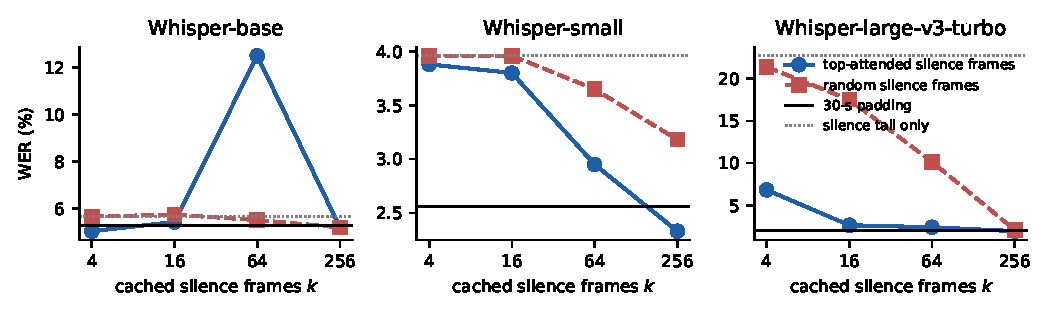
\includegraphics[width=\textwidth]{topk_vs_random.pdf}
    \caption{The encoder's use of silence is concentrated in a few attention-sink positions, and increasingly so with model size. WER when speech queries attend to $k$ cached silence positions chosen by received attention in the silence-only run (blue) or at random (red); the decoder sees the full cached tail in both cases. For large-v3-turbo, 4--16 sink positions recover most of the gap to padded inference, while random positions do not. Pilot, 100 utterances.}
    \label{fig:topk}
\end{figure*}

The top-$k$ results locate the encoder-side effect (Fig.~\ref{fig:topk}). For base and small, the choice of cached positions barely matters, consistent with their weak dependence on encoder-side silence. For large-v3-turbo the gap is large: 16 high-attention positions give 2.64\% WER versus 17.53\% for 16 random ones, and the curves meet only at $k=256$. The highest-attention silence positions are at fixed absolute indices: for large-v3-turbo they are positions 0, 1496, 1499, 1487, 1455, 1495, 1456 and 1494. This suggests why 5\,s of real padding fails for turbo: it never fills the end-of-window positions. We treat this as a hypothesis for the full evaluation (H3d in the project plan).

\subsection{Ablation Study}
\label{sec:ablation}

Two ablations isolate what \method{} relies on. \emph{Registers versus sinks.} Masking or removing the highest-norm frames, the registers in the sense of~\cite{darcet2024registers}, does not change WER (Table~\ref{tab:results}, last rows), whereas restricting the cache to random rather than high-attention positions does. Functional reliance therefore follows received attention, not norm. This agrees with evidence that sinks can exist without massive activations~\cite{sun2026anatomy}. One caveat: in base, the high-attention silence positions include the top-norm frames (positions 1445, 1446, 1453 and 1454), so the overlap between the two sets must be measured per layer before the dissociation is claimed in general (planned experiment E4). \emph{Decoder tail size.} With the full key/value cache, base and small still need many tail positions (14.27\% and 12.34\% WER with only the top-16), while turbo needs very few (1.94\%). How much silence the decoder must see, and whether nearest-first or highest-attention tail positions matter, is the subject of a planned tail-length sweep.

\subsection{Additional Analysis}
\label{sec:additional-analysis}

\paragraph{Partial padding helps gradually, but only in small models.} With real zero padding on Whisper-base, WER falls from 31.2\% with 1\,s to 16.3\% with 2\,s and 5.9\% with 5\,s or 10\,s (\appref{app:supp-results}), whereas large-v3-turbo still has 35.1\% with 5\,s (Table~\ref{tab:results}). Transplanting the keys/values of four register frames from a padded run into an unpadded one does not help (315\% WER), while appending a padding tail from a \emph{speech} reference gives 24.5\%, far worse than the content-free silence tail (5.66\%). The tail must therefore be silence-conditioned, not merely ``padding-shaped''.

\paragraph{Non-speech audio.} On 200 ESC-50 clips~\cite{piczak2015esc} the silence tail shortens runaway outputs but does not prevent short hallucinations. For large-v3-turbo the share of clips with any output is 78.5\% with padding, 98.0\% without, and 100\% with the tail; mean output length is 1.10, 16.27 and 1.32 words respectively. Non-speech hallucination is therefore treated as exploratory (\appref{app:supp-results}).

\paragraph{Planned analyses.} (a) The RQ1 census with entropy and anisotropy per layer. (b) A factorial over the energy, redundancy, position and duration of inserted non-speech blocks, which pits the redundancy~\cite{darcet2024registers}, least-shared~\cite{ngnawe2026spike} and self-sinking~\cite{sun2026anatomy,li2026structural} accounts against each other. (c) Mask-to-self interventions~\cite{li2026structural}. (d) Decoder cross-attention anatomy at end-of-transcript steps. (e) Audio-LLM encoders whose padding is masked or absent. (f) A benchmark against a re-trained hush word~\cite{wang2024whisperflow}, fine-tuned short-context checkpoints, stride-$k$~\cite{cho2026stridek} and combinations.

% ============================================================
% 05. DISCUSSION
% ============================================================
\section{Discussion}
\label{sec:discussion}

The pilot changes the question from ``do speech transformers need registers?'' to ``what does silence do for them?''. Its answer is that Whisper uses silence as a source of attention sinks and end-of-speech evidence, and that the high-norm register tokens, though present, are not what it relies on. The causal language here is limited to interventions on three models and 100 utterances; the full evaluation is designed to test each statement at scale.

\subsection{Interpretation}

Two mechanisms are consistent with the results. On the decoder side, silent encoder states give cross-attention somewhere to go once the transcript is complete. Without them the decoder re-reads the speech and loops, which matches the observation that unpadded failures are dominated by continuations beyond the reference~\cite{lee2026npusper}, and the view that softmax attention needs a sink to realise a default state~\cite{ranmilo2026necessary}. On the encoder side, speech queries of larger models attend to a few silence positions at fixed indices near the window edges. Proposition~\ref{prop:placeholder} explains why such sinks can be cached: what matters to other tokens is the sink's key and value. Their anchoring to absolute positions resembles the first-token sink of causal language models~\cite{sun2026anatomy,li2026structural}, but here it appears at both ends of a bidirectional window. Why it appears there, and why it strengthens with scale, is open. The planned factorial and mask-to-self experiments address it. We label as speculative the idea that end-of-window sinks arise because padding always occupies those positions during training.

\subsection{Limitations}

The pilot uses read English speech, short utterances, greedy decoding and three checkpoints. Long-form decoding with timestamps, beam search, noisy and multilingual speech are untested, and the large-v3 encoder was not yet run. FLOPs are analytic; attention to cached keys may not yield proportional wall-clock gains with all kernels. The cache is computed from digital silence; recordings whose ``silence'' is noise may need a cache matched to the noise floor. The dissociation between sinks and registers depends on how the two sets are selected; this is unresolved where they overlap (e.g.\ base). Finally, \method{} assumes access to model internals, unlike API-only deployments.

\subsection{Broader Implications and Future Work}

If the account holds, three things follow. Any transformer trained with fixed-length padding may learn to depend on it, so removing padding should preserve its sinks rather than simply truncate. Analyses of speech representations should report silence handling, because massive activations and sinks on silent frames dominate norms and attention statistics. And audio language models built on Whisper encoders inherit, mask or lose these sinks depending on their padding regime, which may matter for audio-token pruning and hallucination. Future work includes the audio-LLM natural experiment, streaming with cached sinks, and training-time interventions (explicit silence registers or gated attention~\cite{qiu2025gated}) that would make speech models robust to variable-length input by design.

% ============================================================
% 06. CONCLUSION
% ============================================================
\section{Conclusion}
\label{sec:conclusion}

Whisper fails without its 30\,s padding, and we asked what the silence is used for. Pilot interventions on three Whisper sizes show that the high-norm register tokens the encoder forms on padding are dispensable, while silence serves two roles that are not: end-of-speech evidence for the decoder and a few position-anchored attention sinks for the encoder, whose importance grows with model size. Caching these silence states once gives \method{}, a training-free way to encode only the speech, which matched or improved padded WER at about one sixth of the encoder FLOPs in the pilot. These conclusions rest on 100 utterances per model; the specified full-scale evaluation will determine how far they generalise across sizes, languages, conditions and audio language models.


% ============================================================
% Optional acknowledgments
% ============================================================
\begin{acknowledgments}
To be completed. Pilot experiments ran on a single NVIDIA RTX 3050 Laptop GPU (4\,GB); full-scale experiments are planned on Kaggle T4 GPUs.
\end{acknowledgments}

% ============================================================
% Bibliography
% ============================================================
\bibliographystyle{apsrev4-2}
\bibliography{ref}

% ============================================================
% Optional appendices kept in a separate file as well
% ============================================================
% ============================================================
% APPENDICES
% The main text cites these with the section-sign style, e.g., \appref{app:notation} (rendered as \S A).
% ============================================================
\clearpage
\onecolumngrid
\appendix

\section{Notation and Symbols}
\label{app:notation}

This section collects the notation used in the paper. The WER is defined in \eqnref{eq:objective}, attention in \eqnref{eq:loss}, the cached keys/values of \method{} in \eqnref{eq:update}, the hallucination rate in \eqnref{eq:accuracy} and the per-layer cost in \eqnref{eq:cost}.

\begin{small}
\begin{description}
    \item[$N=1500$] Number of Whisper encoder positions in a 30\,s window (20\,ms each).
    \item[$T$] Encoder positions covered by the utterance, $T=\lceil 50\tau\rceil$ for duration $\tau$ in seconds.
    \item[$L$, $d$, $f$] Number of encoder layers, model width and MLP width ($f=4d$).
    \item[$\mathbf{X}^{(\ell)}$, $\mathbf{x}^{(\ell)}_j$] Hidden states of layer $\ell$ (before the final LayerNorm) and the state at position $j$.
    \item[$\mathbf{q}_i,\mathbf{k}_j,\mathbf{v}_j$, $a_{ij}$] Query, key, value and attention weight of a head.
    \item[$\bar a_j$] Received attention of position $j$, averaged over heads and queries.
    \item[$\Psi^{(\ell)}$] Ratio of the largest to the median absolute activation in layer $\ell$.
    \item[$\mathbf{K}^{(\ell)}_{\varnothing},\mathbf{V}^{(\ell)}_{\varnothing}$] Keys and values of layer $\ell$ for a 30\,s silence input.
    \item[$\mathbf{S}$] Encoder outputs for the silence input; $\mathbf{S}_{T+1:N}$ is the ``tail''.
    \item[$\mathcal{C}$, $\mathcal{D}$] Cached silence positions used as extra keys (encoder) and as extra memory (decoder).
    \item[$\mathbf{H}$] Encoder outputs given to the decoder.
    \item[$C(T_q,T_k)$] FLOPs of one encoder layer with $T_q$ queries and $T_k$ keys.
    \item[$\mathrm{WER}$, $\mathrm{Hal}$] Word error rate and hallucination rate (\%).
\end{description}
\end{small}

\section{Additional Derivations}
\label{app:derivations}

\paragraph{Encoder cost.} A pre-LN block applies four $d\times d$ projections (query, key, value, output) and a two-layer MLP of width $f$ to each of the $T_q$ query positions, i.e.\ $T_q(4d^2+2df)$ multiply--accumulates. Attention scores and the weighted sum of values each need $T_qT_kd$ multiply--accumulates. Counting a multiply--accumulate as two FLOPs gives
\begin{align}
    C(T_q,T_k)
    &= 2T_q(4d^2+2df) + 2\cdot 2\,T_qT_kd \\
    &= 2T_q(4d^2+2df) + 4\,T_qT_kd ,
\end{align}
which is \eqnref{eq:cost}; the key/value projections for cached positions are computed once offline and are excluded. Layer norms, the convolutional stem (which processes only the $2T$ unpadded mel frames under \method{}) and the softmax are lower order. With a full cache every speech query sees exactly $N$ keys (its own $T$ plus the $N-T$ cached ones), so the relative cost of \method{} is
\begin{equation}
    \rho_{\mathrm{full}}=\frac{C(T,N)}{C(N,N)}=\frac{T\,[2(4d^2+2df)+4Nd]}{N\,[2(4d^2+2df)+4Nd]}=\frac{T}{N}.
\end{equation}
The pilot's mean $T$ is 234.4 positions, so $\rho_{\mathrm{full}}=0.156$, matching the reported 0.157 (averaged per utterance). With a top-$k$ cache the attention term shrinks to $4T(T{+}k)d$, and $C(T,T{+}k)/C(N,N)$ approaches the cost of unpadded encoding (0.11--0.14 in the pilot).

\section{Implementation and Reproducibility Details}
\label{app:implementation}

All code is in the project repository (\texttt{experiments/pilot\_padding}). The encoder forward pass is written explicitly from the checkpoint weights and checked against the Hugging Face implementation (maximum absolute difference $6.9\times10^{-4}$ at output scale 23.6 on a padded utterance; identical greedy transcript). Log-mel features use the official feature extractor without padding, with the waveform zero-extended to a multiple of 320 samples so that the number of encoder positions is an integer. Sinusoidal position embeddings are sliced to the first $T$ positions. Cached keys and values are taken at positions $[T{+}1,N]$ of the silence run, so every speech query sees each absolute position at most once.

\begin{table}[!htbp]
\centering
\small
\setlength{\tabcolsep}{8pt}
\caption{Software and settings of the pilot.}
\label{tab:implementation}
\begin{tabular}{l l}
\toprule
\textbf{Item} & \textbf{Setting} \\
\midrule
Software & Python 3.14, PyTorch 2.11 (CUDA 12.8), Transformers 5.19, jiwer \\
Checkpoints & \texttt{openai/whisper-base}, \texttt{-small}, \texttt{-large-v3-turbo} \\
Precision & fp32 (base, small); fp16 (turbo) \\
Decoding & greedy; special tokens above end-of-text suppressed; 160 tokens max \\
Text normalisation & Whisper English normaliser (\texttt{tokenizer.normalize}) \\
Utterance selection & 2--8\,s test-clean utterances, shuffled with seed 0, first 100 \\
Register frames & top-$k$ token norm at the block after the emergence block \\
Sink frames & top-$k$ received attention (all layers, heads, queries) in the silence run \\
Hardware & NVIDIA RTX 3050 Laptop GPU, 4\,GB \\
\bottomrule
\end{tabular}
\end{table}

The full evaluation will add bootstrap confidence intervals (1{,}000 resamples), paired tests, wall-clock measurements with CUDA events and peak-memory reports, and will fix all selection rules before running on the test sets.

\FloatBarrier

\section{Supplementary Results and Analyses}
\label{app:supp-results}

\begin{table}[!htbp]
\centering
\small
\setlength{\tabcolsep}{8pt}
\caption{Whisper-base with real partial zero padding and register transplants (pilot v1, same 100 utterances; WER \%).}
\label{tab:supp-results}
\begin{tabular}{l c}
\toprule
\textbf{Condition} & \textbf{WER} \\
\midrule
30\,s padding & 5.39 \\
no padding & 385.46 \\
1 / 2 / 5 / 10\,s padding & 31.20 / 16.34 / 5.94 / 5.86 \\
no padding + tail from a \emph{speech} reference & 24.47 \\
no padding + 4 transplanted register keys/values & 315.40 \\
both & 25.02 \\
padded; encoder attention to own 4 register frames masked & 5.39 \\
\bottomrule
\end{tabular}
\end{table}

\begin{table}[!htbp]
\centering
\small
\setlength{\tabcolsep}{6pt}
\caption{Top-$k$ versus random-$k$ cached silence positions (KV + full tail; WER \%; pilot).}
\label{tab:topk-full}
\begin{tabular}{l cccc cccc}
\toprule
 & \multicolumn{4}{c}{\textbf{top-$k$}} & \multicolumn{4}{c}{\textbf{random-$k$}} \\
\cmidrule(lr){2-5}\cmidrule(lr){6-9}
Model & 4 & 16 & 64 & 256 & 4 & 16 & 64 & 256 \\
\midrule
Whisper-base & 5.04 & 5.43 & 12.49$^\ast$ & 5.20 & 5.66 & 5.74 & 5.51 & 5.20 \\
Whisper-small & 3.88 & 3.80 & 2.95 & 2.33 & 3.96 & 3.96 & 3.65 & 3.18 \\
Whisper-large-v3-turbo & 6.83 & 2.64 & 2.40 & 1.94 & 21.41 & 17.53 & 10.16 & 2.09 \\
\bottomrule
\end{tabular}

\vspace{2pt}{\footnotesize $^\ast$Single outlier cell, to be re-checked at scale.}
\end{table}

\begin{table}[!htbp]
\centering
\small
\setlength{\tabcolsep}{6pt}
\caption{Non-speech audio (ESC-50, 200 clips; pilot v3). Share of clips with any output word (\%) and mean output words.}
\label{tab:esc}
\begin{tabular}{l cc cc}
\toprule
 & \multicolumn{2}{c}{\textbf{Whisper-base}} & \multicolumn{2}{c}{\textbf{Whisper-large-v3-turbo}} \\
\cmidrule(lr){2-3}\cmidrule(lr){4-5}
Condition & any output & words & any output & words \\
\midrule
clip + 25\,s padding & 1.0 & 0.80 & 78.5 & 1.10 \\
clip only & 8.5 & 1.37 & 98.0 & 16.27 \\
clip only + silence tail & 5.0 & 0.06 & 100.0 & 1.32 \\
clip tiled to 30\,s & 3.0 & 1.05 & 94.0 & 2.81 \\
clip tiled to 25\,s + 5\,s padding & 4.5 & 1.60 & 87.5 & 6.30 \\
\bottomrule
\end{tabular}
\end{table}

These tables extend the main pilot with the same protocol. Additional robustness results (noise, long-form, beam search, languages) will be added from the full evaluation described in Sec.~\ref{sec:evaluation}.


\end{document}
